% \section{Neutron Stars and Nuclear Matter}%
% \label{sec:neutron_stars_and_nuclear_matter}

Neutron stars (\gls{NS}) are star-like astronomical objects with mass $M$ on the order of solar mass ($M_\odot$), a radius of $\sim 10-12\;km$ and an average density $n$ several times greater than that of nucleon ($\rho_0 \approx 0.16\;fm^{-3}$). They are arguably the densest accessible objects, excluding black holes which we know nothing about inside the event horizon, in the universe \citep{baym1975neutron}. Due to extremely high density, the matter on \gls{NS} mainly consists of neutrons that are closely packed together with a small percentage of other particles ($p$, $e^-$, \ldots), similar to a atomic nucleus on macroscopic scale. For this reason, they are also the ideal objects for testing physical theories of dense matter and provide connections between different field of physics, i.e. nuclear physics, elementary particle physics and astrophysics \citep{lattimer2004physics}.\par
During the \gls{NS}'s formation process, protons ($p$) and electrons ($e^-$) combined together to form neutrons, i.e.
\begin{equation}
        p + e^- \longrightarrow n + \nu_e
\end{equation}
and the star only holds itself against gravity by its own degeneracy pressure and strong force repulsion, which explains why the matter on \gls{NS} is neutron-dominant and hence the name ``neutron stars''. After the \gls{NS} is formed, energy quickly dissipates through neutrino emission, resulting in a relatively cold \gls{NS}. In this study, we will only concern with the \gls{NS} after a considerable time from its formation, when the temperature is considered to be $T=0\;K$.\par
On a \gls{NS}, the matter exists as an inhomogenous, low-density \emph{crust} and gradually becomes a more uniform \emph{core} the closer to the \gls{NS} center as in Figure \ref{fig:NS_structure}. In order to study about the properties of \gls{NS} matter, the problem have to be approached from the nuclear physics point of view, where we study about \emph{nuclear matter} (\gls{NM}). For a nuclear system as massive as a \gls{NS}, we consider one with infinite number of nucleons that are in \textbeta-stable state with a small portion of leptons, in which the properties of matter are described using an \emph{equation of states} (\gls{EoS}), i.e. the relation between different state variables (pressure $P$, mass-energy density $\varepsilon$, \ldots) of the system. Ideally, the \gls{EoS} can be derived from the interactions of quarks under strong force in the framework of quantum chromodynamics. However, due to this having yet to be possible at the moment, the \gls{EoS} of \gls{NM} is instead interpreted from a nonrelativistic mean-field study approach with several updated versions of the realistic density-dependent CDM3Y$n$ interaction models \citep{khoa1995equation,khoa2007mean} using Hartree-Fock (\gls{HF}) formalism, which will be implemented further in Chapter \ref{chap:hf}.

\begin{figure}[t]
        \centering
        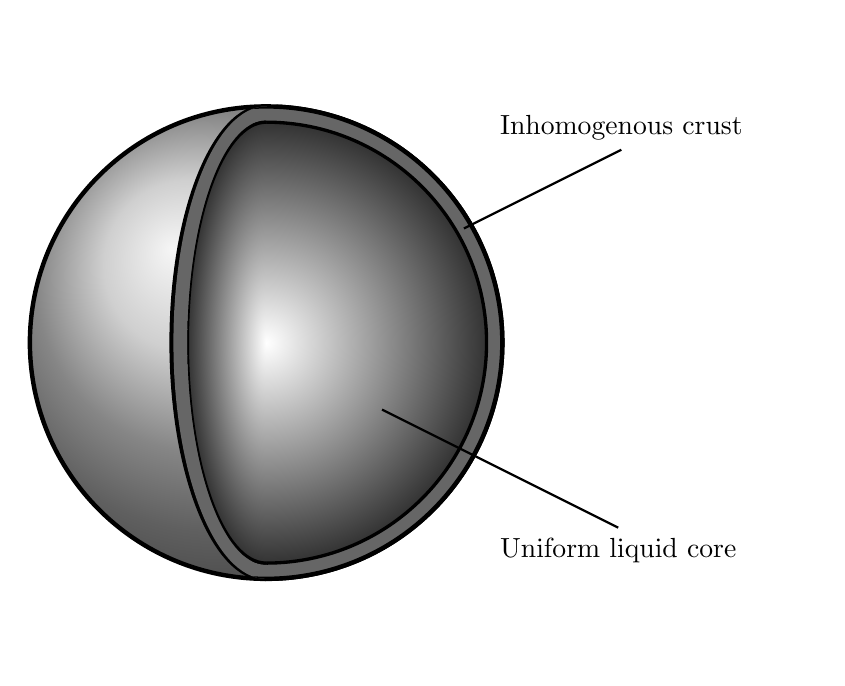
\begin{tikzpicture}[scale=1]
                \draw[ball color=gray!50,shading=ball, ultra thick, color=black] (0,0) circle (3cm);
                \draw[ultra thick] (0,3) arc (90:270:1.2cm and 3cm);
                \clip (0,-3) -- ++(7,-1) -- ++(0,8) -- ++(-7,-1) arc (90:270:1.177cm and 3cm) -- cycle;
                \draw[fill=gray!80!black, ultra thick] (0,0) circle (3cm); 
                \clip (0,-2.82) -- ++(7,-1) -- ++(0,7.64) -- ++(-7,-1) arc (90:270:1cm and 2.82cm) -- cycle;
                \shadedraw[draw=black, very thick,inner color=white, outer color=black!80] (0,0) circle (2.8cm);
                \draw[thick] (30:2.9cm) -- ++(2,1) node[above]{Inhomogenous crust};
                \draw[thick] (-30:1.7cm) -- ++(3,-1.5) node[below]{Uniform liquid core};
                \clip (0,2.82) arc (90:270:1.05cm and 2.82cm) -- cycle;
                \shadedraw[draw=black, very thick, inner color=white, outer color=black!80] (0,0) ellipse (1cm and 2.8cm);
        \end{tikzpicture}
        \caption{Neutron star's overall structure. The baryon density decreases (from white to dark gray) as we move outward from the \gls{NS} center.}
        \label{fig:NS_structure}
\end{figure} 

% \section{Tidal Deformation of Neutron Stars}%
% \label{sec:tidal_deformation_of_neutron_stars}

Following the gravitational wave (\gls{GW}) signals GW170817 \citep{abbott2017gw170817} and GW190425 \citep{abbott2020gw190425} from two binary \gls{NS} mergers observed by LIGO and Virgo laser interferometer in 17\textsuperscript{th} August 2017 and 25\textsuperscript{th} April 2019 respectively, the tidal deformation of the \gls{NS} can be further constrained, as well as the mass $M$ and radius $R$ of the \gls{NS} \citep{abbott2018gw170817}. The \gls{NS} merger event is illustrated as in Figure \ref{fig:NS_merger}.

\begin{figure}[t]
        \centering
        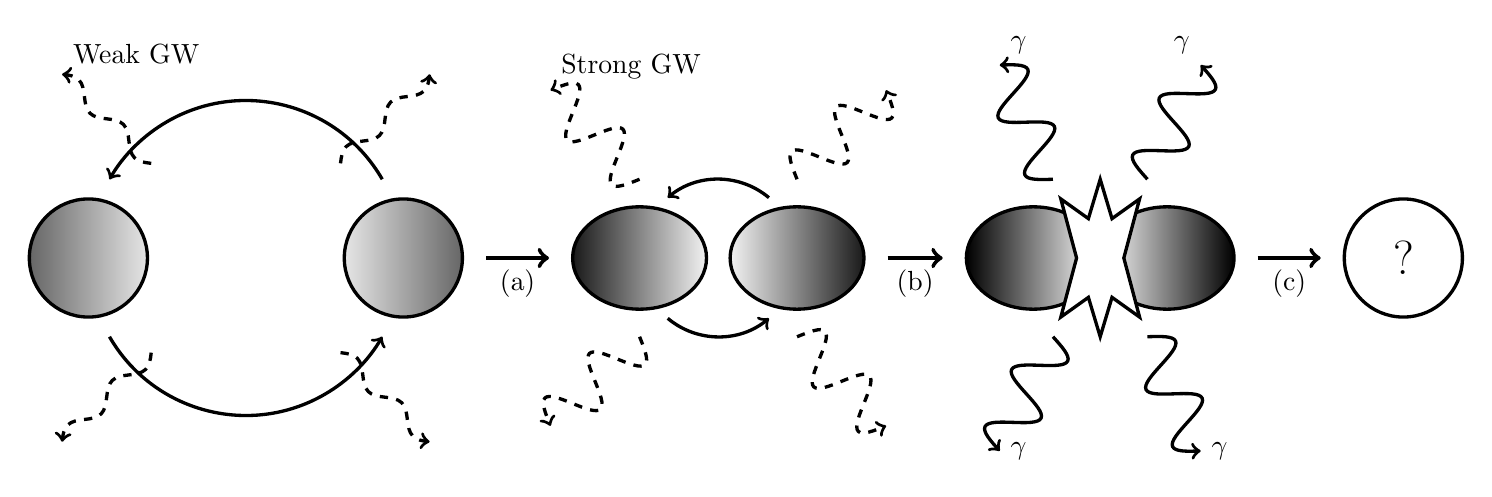
\begin{tikzpicture}[scale=1]
                \def\xl{-2};
                \def\xr{2};
                \def\r{0.75};
                \def\sep{3};
                \shadedraw[very thick, draw=black,left color=gray!80!black, right color=gray!20!white] (\xl,0) circle (\r cm);
                \shadedraw[very thick, draw=black,right color=gray!80!black, left color=gray!20!white] (\xr,0) circle (\r cm);
                \draw[->, very thick] (30:\xr cm) arc (30:150:\xr cm);
                \draw[->, very thick] (210:\xr cm) arc (210:330:\xr cm);
                \def\ang{-45};
                \draw[dashed, ->, very thick, cm={cos(\ang),-sin(\ang),sin(\ang),cos(\ang), (-\ang:1.7 cm)}] (0,0) sin (0.2,0.1) cos (0.4,0) sin (0.6,-0.1) cos (0.8,0) sin (1,0.1) cos (1.2,0) sin (1.4,-0.1) cos (1.6,0);
                \def\ang{-135};
                \draw[dashed, ->, very thick, cm={cos(\ang),-sin(\ang),sin(\ang),cos(\ang), (-\ang:1.7 cm)}] (0,0) sin (0.2,0.1) cos (0.4,0) sin (0.6,-0.1) cos (0.8,0) sin (1,0.1) cos (1.2,0) sin (1.4,-0.1) cos (1.6,0) node[above right]{Weak \gls{GW}};
                \def\ang{-225};
                \draw[dashed, ->, very thick, cm={cos(\ang),-sin(\ang),sin(\ang),cos(\ang), (-\ang:1.7 cm)}] (0,0) sin (0.2,0.1) cos (0.4,0) sin (0.6,-0.1) cos (0.8,0) sin (1,0.1) cos (1.2,0) sin (1.4,-0.1) cos (1.6,0);
                \def\ang{-315};
                \draw[dashed, ->, very thick, cm={cos(\ang),-sin(\ang),sin(\ang),cos(\ang), (-\ang:1.7 cm)}] (0,0) sin (0.2,0.1) cos (0.4,0) sin (0.6,-0.1) cos (0.8,0) sin (1,0.1) cos (1.2,0) sin (1.4,-0.1) cos (1.6,0);
                \draw[->, ultra thick] (\xr+\r+0.3,0) -- +(\sep-2*\r-0.7,0) node[pos=0.5,below]{(a)};

                \shadedraw[very thick, draw=black,left color=gray!20!black, right color=gray!10!white] (\xr+\sep,0) ellipse (0.85 cm and 0.65 cm);
                \shadedraw[very thick, draw=black,right color=gray!20!black, left color=gray!10!white] (\xr+\sep+2,0) ellipse (0.85 cm and 0.65 cm);
                \def\P{\xr+\sep+1};
                \def\R{1};
                \draw[->, very thick] (\P,0)+(50:\R cm) arc (50:130:\R cm);
                \draw[->, very thick] (\P,0)+(230:\R cm) arc (230:310:\R cm);
                \def\ang{-45};
                \draw[dashed, ->, very thick, cm={cos(\ang),-sin(\ang),sin(\ang),cos(\ang), (\P+1,1)}] (0,0) sin (0.2,0.3) cos (0.4,0) sin (0.6,-0.3) cos (0.8,0) sin (1,0.3) cos (1.2,0) sin (1.4,-0.3) cos (1.6,0);
                \def\ang{-135};
                \draw[dashed, ->, very thick, cm={cos(\ang),-sin(\ang),sin(\ang),cos(\ang), (\P-1,1)}] (0,0) sin (0.2,0.3) cos (0.4,0) sin (0.6,-0.3) cos (0.8,0) sin (1,0.3) cos (1.2,0) sin (1.4,-0.3) cos (1.6,0) node[above right]{Strong \gls{GW}};
                \def\ang{-225};
                \draw[dashed, ->, very thick, cm={cos(\ang),-sin(\ang),sin(\ang),cos(\ang), (\P-1,-1)}] (0,0) sin (0.2,0.3) cos (0.4,0) sin (0.6,-0.3) cos (0.8,0) sin (1,0.3) cos (1.2,0) sin (1.4,-0.3) cos (1.6,0);
                \def\ang{-315};
                \draw[dashed, ->, very thick, cm={cos(\ang),-sin(\ang),sin(\ang),cos(\ang), (\P+1,-1)}] (0,0) sin (0.2,0.3) cos (0.4,0) sin (0.6,-0.3) cos (0.8,0) sin (1,0.3) cos (1.2,0) sin (1.4,-0.3) cos (1.6,0);
                \draw[->, ultra thick] (\xr+\sep+2.85+0.3,0) -- +(\sep-2*0.85-0.6,0) node[pos=0.5,below]{(b)};

                \shadedraw[very thick, draw=black,left color=gray!0!black, right color=gray!0!white] (\xr+2*\sep+2,0) ellipse (0.85 cm and 0.65 cm);
                \shadedraw[very thick, draw=black,right color=gray!0!black, left color=gray!0!white] (\xr+2*\sep+3.7,0) ellipse (0.85 cm and 0.65 cm);
                \draw[->, ultra thick] (\xr+2*\sep+3.7+0.85+0.3,0) -- +(\sep-\r-0.85-0.6,0) node[pos=0.5,below]{(c)};
                \def\P{\xr+2*\sep+2.85};
                \draw[fill=white, very thick, shift={(\P,0)}] (0,1) -- (0.15,0.5) -- (0.5, 0.75) -- (0.3,0) -- (0.5,-0.75) -- (0.15,-0.5) -- (0,-1) -- (-0.15,-0.5) -- (-0.5,-0.75) -- (-0.3,0) -- (-0.5,0.75) -- (-0.15,0.5) -- cycle;
                \def\ang{-65};
                \draw[->, very thick, cm={cos(\ang),-sin(\ang),sin(\ang),cos(\ang), (\P+0.6,1)}] (0,0) sin (0.2,0.3) cos (0.4,0) sin (0.6,-0.3) cos (0.8,0) sin (1,0.3) cos (1.2,0) sin (1.4,-0.3) cos (1.6,0) node[above left]{$\gamma$};
                \def\ang{-115};
                \draw[->, very thick, cm={cos(\ang),-sin(\ang),sin(\ang),cos(\ang), (\P-0.6,1)}] (0,0) sin (0.2,0.3) cos (0.4,0) sin (0.6,-0.3) cos (0.8,0) sin (1,0.3) cos (1.2,0) sin (1.4,-0.3) cos (1.6,0) node[above right]{$\gamma$};
                \def\ang{-245};
                \draw[->, very thick, cm={cos(\ang),-sin(\ang),sin(\ang),cos(\ang), (\P-0.6,-1)}] (0,0) sin (0.2,0.3) cos (0.4,0) sin (0.6,-0.3) cos (0.8,0) sin (1,0.3) cos (1.2,0) sin (1.4,-0.3) cos (1.6,0) node[right]{$\gamma$};
                \def\ang{-295};
                \draw[->, very thick, cm={cos(\ang),-sin(\ang),sin(\ang),cos(\ang), (\P+0.6,-1)}] (0,0) sin (0.2,0.3) cos (0.4,0) sin (0.6,-0.3) cos (0.8,0) sin (1,0.3) cos (1.2,0) sin (1.4,-0.3) cos (1.6,0) node[right]{$\gamma$};

                \draw[very thick] (\xr+3.7+2*\sep+\sep,0) circle (\r cm) node{\LARGE ?};
        \end{tikzpicture}
        \caption{Illustration of binary \gls{NS} merger. (a) The two companion \glspl{NS} orbit about each others, while gradually losing energy through weak \gls{GW} and come closer with time. (b) As the two \gls{NS} get closer, they accelerate and emit stronger \gls{GW} until (c) colliding, which results in a \emph{kilonova}, characterized by a short \emph{gamma ray burst} (\gls{GRB}). The product of the merger has yet been decided to be a black hole (\gls{BH}) or another \gls{NS}.}
        \label{fig:NS_merger}
\end{figure} 
Apparently, the \gls{EoS} of high-density \gls{NM} plays the most important role in deciding the macroscopic properties of \gls{NS}. In particular, given the \gls{EoS} of the crust from the compressible liquid drop model and by using the \gls{EoS} of the uniform \gls{NS} core from the result of the \gls{HF} calculation of cold \textbeta-stable \gls{NM}, the gravitational mass and radius of the star can be decided by the framework of General Relativity (\gls{GR}) \citep{tan2020spin,tan2021equation}, i.e. the Tolman-Oppenheimer-Volkoff (\gls{TOV}) equation, which will in turn be compared to the observational astrophysical constraints to deduce the most suitable \gls{EoS} of the constituent \gls{NS} in this system.\par
In addition, due to the enormous mass, each \gls{NS} possesses powerful gravitational field and therefore, they tend to ``stretch out'' their companion under the tidal effect as in Figure \ref{fig:NS_merger}, while orbiting spirally toward each others and dissipating energy under the form of \gls{GW}. Particularly, the shape and mass-energy distribution of the \gls{NS} are tidally deformed from its supposedly spherical shape, resulting in nonzero multipole moments \citep{hinderer2008tidal,hinderer2010tidal,damour2009relativistic}. The \gls{NS}'s reaction, i.e. how strongly it deforms when being under a tidal field, is expressed in terms of the \emph{tidal Love numbers} $k_l$ of several orders $l$, where in this study, we will evaluate the Love number of \gls{NS} up to the 4\textsuperscript{th} order, i.e. $l=2,3,4$ \citep{perot2021role}. Apparently, the tidal Love number depends heavily on the \gls{EoS} of matter and this dependence will be further emphasized in Chapter \ref{chap:ns_prop}. For \gls{NS}, the central density can be up to $6\rho_0$ and possesses a Love number of order $\sim 0.1$, while our Earth has that of $0.3$. In a recent study, the Love number was calculated for spinning black holes, which showed that even with nearly infinite density, they still posess a small Love number of $0.002$ \citep{le2021spinning}.\par
Furthermore, under small perturbation of spacetime, the tidal field can also be separated into two components: the \emph{gravito-electric} (\gls{GE}) and \emph{gravito-magnetic} (\gls{GM}) terms \citep{damour2009relativistic} that are analogous to that in eletromagnetic field. As a result, the deformation of the \gls{NS}, i.e. Love numbers, in the perturbed tidal field can also be categorized into the corresponding \gls{GE} ($k_l$) and \gls{GM} ($j_l$) components \citep{perot2021role}, whose result will be presented in more details in Chapter \ref{chap:ns_prop}. To sum up, this study is dedicated to:
\begin{itemize}
        \item Include the spin polarization effect to the existing CDM3Y$n$ models \citep{tan2021equation},
        \item Assess the dependence of \gls{NS}'s gravitational mass and radius to different \gls{EoS},
        \item Investigate the sensitivity of \gls{GE} and \gls{GM} tidal deformability and Love numbers to \gls{NM} properties,
        \item Compare the \gls{NS}'s calculated properties to the astrophysical constraints obtained experimentally.
\end{itemize}
